%%%%%%%%%%%%%%%%%%%%%%%%%%%%%%%%%%%%%%%%%
% Programming/Coding Assignment
% LaTeX Template
%
% This template has been downloaded from:
% http://www.latextemplates.com
%
% Original author:
% Ted Pavlic (http://www.tedpavlic.com)
%
% Note:
% The \lipsum[#] commands throughout this template generate dummy text
% to fill the template out. These commands should all be removed when 
% writing assignment content.
%
% This template uses a Perl script as an example snippet of code, most other
% languages are also usable. Configure them in the "CODE INCLUSION 
% CONFIGURATION" section.
%
%%%%%%%%%%%%%%%%%%%%%%%%%%%%%%%%%%%%%%%%%

%----------------------------------------------------------------------------------------
%	PACKAGES AND OTHER DOCUMENT CONFIGURATIONS
%----------------------------------------------------------------------------------------

\documentclass{article}

\usepackage{fancyhdr} % Required for custom headers
\usepackage{lastpage} % Required to determine the last page for the footer
\usepackage{extramarks} % Required for headers and footers
\usepackage[usenames,dvipsnames]{color} % Required for custom colors
\usepackage{graphicx} % Required to insert images
\usepackage{listings} % Required for insertion of code
\usepackage{courier} % Required for the courier font
\usepackage{lipsum} % Used for inserting dummy 'Lorem ipsum' text into the template
\usepackage{amsmath}
\usepackage{amssymb}
\usepackage{mathtools, xparse}
\usepackage{booktabs}
\usepackage{bigstrut}
\usepackage{float}
\usepackage{hyperref}
\usepackage{color}
\usepackage{algorithm}
\usepackage{caption}
\usepackage{algpseudocode}
\usepackage{multirow}


\DeclarePairedDelimiter{\norm}{\lVert}{\rVert}
\DeclarePairedDelimiter\abs{\lvert}{\rvert}%

\hypersetup{
    colorlinks   = true,    % Colours links instead of ugly boxes
    urlcolor     = red,    % Colour for external hyperlinks
    linkcolor    = red,    % Colour of internal links
    citecolor    = red      % Colour of citations
}
% Margins
\topmargin=-0.45in
\evensidemargin=0in
\oddsidemargin=0in
\textwidth=6.5in
\textheight=9.0in
\headsep=0.25in

\linespread{1.1} % Line spacing

% Set up the header and footer
\pagestyle{fancy}
\lhead{\hmwkAuthorName} % Top left header
\chead{\hmwkClass\ : \hmwkID} % Top center head
\rhead{\firstxmark} % Top right header
\lfoot{\lastxmark} % Bottom left footer
\cfoot{} % Bottom center footer
\rfoot{Page\ \thepage\ of\ \protect\pageref*{LastPage}} % Bottom right footer
\renewcommand\headrulewidth{0.4pt} % Size of the header rule
\renewcommand\footrulewidth{0.4pt} % Size of the footer rule

\setlength\parindent{0pt} % Removes all indentation from paragraphs

%----------------------------------------------------------------------------------------
%	CODE INCLUSION CONFIGURATION
%----------------------------------------------------------------------------------------

\definecolor{MyDarkGreen}{rgb}{0.0,0.4,0.0} % This is the color used for comments
\lstloadlanguages{Perl} % Load Perl syntax for listings, for a list of other languages supported see: ftp://ftp.tex.ac.uk/tex-archive/macros/latex/contrib/listings/listings.pdf
\lstset{language=Perl, % Use Perl in this example
    frame=single, % Single frame around code
    basicstyle=\small\ttfamily, % Use small true type font
    keywordstyle=[1]\color{Blue}\bf, % Perl functions bold and blue
    keywordstyle=[2]\color{Purple}, % Perl function arguments purple
    keywordstyle=[3]\color{Blue}\underbar, % Custom functions underlined and blue
    identifierstyle=, % Nothing special about identifiers                                         
    commentstyle=\usefont{T1}{pcr}{m}{sl}\color{MyDarkGreen}\small, % Comments small dark green courier font
    stringstyle=\color{Purple}, % Strings are purple
    showstringspaces=false, % Don't put marks in string spaces
    tabsize=5, % 5 spaces per tab
    %
    % Put standard Perl functions not included in the default language here
    morekeywords={rand},
    %
    % Put Perl function parameters here
    morekeywords=[2]{on, off, interp},
    %
    % Put user defined functions here
    morekeywords=[3]{test},
    %
    morecomment=[l][\color{Blue}]{...}, % Line continuation (...) like blue comment
    numbers=left, % Line numbers on left
    firstnumber=1, % Line numbers start with line 1
    numberstyle=\tiny\color{Blue}, % Line numbers are blue and small
    stepnumber=5 % Line numbers go in steps of 5
}

% Creates a new command to include a perl script, the first parameter is the filename of the script (without .pl), the second parameter is the caption
\newcommand{\perlscript}[2]{
    \begin{itemize}
        \item[]\lstinputlisting[caption=#2,label=#1]{#1.py}
    \end{itemize}
}
\newcommand{\cppscript}[1]{
    \begin{itemize}
        \item[]\lstinputlisting[]{#1}
    \end{itemize}
}

%----------------------------------------------------------------------------------------
%	DOCUMENT STRUCTURE COMMANDS
%	Skip this unless you know what you're doing
%----------------------------------------------------------------------------------------

% Header and footer for when a page split occurs within a problem environment
\newcommand{\enterProblemHeader}[1]{
    \nobreak\extramarks{#1}{#1 continued on next page\ldots}\nobreak
    \nobreak\extramarks{#1 (continued)}{#1 continued on next page\ldots}\nobreak
}

% Header and footer for when a page split occurs between problem environments
\newcommand{\exitProblemHeader}[1]{
    \nobreak\extramarks{#1 (continued)}{#1 continued on next page\ldots}\nobreak
    \nobreak\extramarks{#1}{}\nobreak
}

%\setcounter{secnumdepth}{0} % Removes default section numbers
\newcounter{homeworkProblemCounter} % Creates a counter to keep track of the number of problems

\newcommand{\homeworkProblemName}{}
\newenvironment{homeworkProblem}[1][Problem \arabic{homeworkProblemCounter}]{ % Makes a new environment called homeworkProblem which takes 1 argument (custom name) but the default is "Problem #"
    \stepcounter{homeworkProblemCounter} % Increase counter for number of problems
    \renewcommand{\homeworkProblemName}{#1} % Assign \homeworkProblemName the name of the problem
    \section{\homeworkProblemName} % Make a section in the document with the custom problem count
    \enterProblemHeader{\homeworkProblemName} % Header and footer within the environment
    }{
    \exitProblemHeader{\homeworkProblemName} % Header and footer after the environment
}

\newcommand{\problemAnswer}[1]{ % Defines the problem answer command with the content as the only argument
\noindent\framebox[\columnwidth][c]{\begin{minipage}{0.98\columnwidth}#1\end{minipage}} % Makes the box around the problem answer and puts the content inside
}

\newcommand{\homeworkSectionName}{}
\newenvironment{homeworkSection}[1]{ % New environment for sections within homework problems, takes 1 argument - the name of the section
    \renewcommand{\homeworkSectionName}{#1} % Assign \homeworkSectionName to the name of the section from the environment argument
    \subsection{\homeworkSectionName} % Make a subsection with the custom name of the subsection
    \enterProblemHeader{\homeworkProblemName\ [\homeworkSectionName]} % Header and footer within the environment
    }{
    \enterProblemHeader{\homeworkProblemName} % Header and footer after the environment
}

%----------------------------------------------------------------------------------------
%	NAME AND CLASS SECTION
%----------------------------------------------------------------------------------------

\newcommand{\hmwkID}{homework 04} % Assignment title
\newcommand{\hmwkTitle}{Linear Iterative Methods}
\newcommand{\hmwkDueDate}{Tuesday,\ March\ 28,\ 2017} % Due date
\newcommand{\hmwkClass}{Numerical Analysis} % Course/class
\newcommand{\hmwkClassTime}{10:30am} % Class/lecture time
\newcommand{\hmwkClassInstructor}{Jones} % Teacher/lecturer
\newcommand{\hmwkAuthorName}{102061149 Fu-En Wang} % Your name

%----------------------------------------------------------------------------------------
%	TITLE PAGE
%----------------------------------------------------------------------------------------

\title{
    \vspace{2in}
    \textmd{\textbf{\hmwkClass}}\\
    \textmd{\textbf{\hmwkID: \hmwkTitle}} \\
    \normalsize\vspace{0.1in}\small{Due\ on\ \hmwkDueDate}\\
    \vspace{3in}
}

\author{\textbf{\hmwkAuthorName}}
\date{} % Insert date here if you want it to appear below your name

%----------------------------------------------------------------------------------------

\begin{document}

\maketitle
\newpage

\section{Introduction}
To solve such linear system:
\begin{gather}
    Ax = b
\end{gather}
We had used \textbf{LU Decomposition} to get $x$ in previous homework. In this project, we will solve it with the following 
iterative methods:
\begin{enumerate}
    \item \textbf{Jacobi Method}
    \item \textbf{Gauss-Seidel Method}
    \item \textbf{Symmetric Gauss-Seidel Method}
\end{enumerate}
To evaluate the performance of three method, we will use Question.4 in previous homework(20 resistors at each side).
\begin{figure}[H]
    \centering
    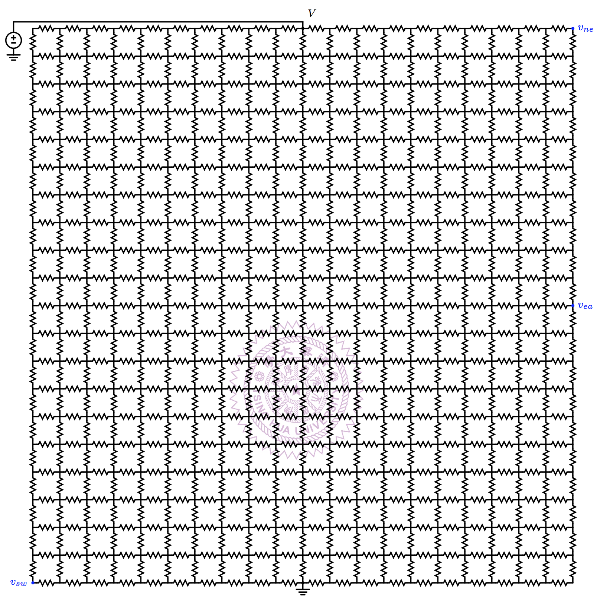
\includegraphics[width=0.6\textwidth]{src/network_small.png}
    \caption{Simple resistor network}
\end{figure}
To calculate the error, we will use the following error formula:
\begin{enumerate}
    \item $ \norm{x}_1 = \sum_{i=1}^{n}\abs{x_i} $
    \item $ \norm{x}_2 = (\sum_{i=1}^{n}x_i^2)^{\frac{1}{2}} $
    \item $ \norm{x}_\infty = max_{i=1}^{n}\abs{x_i}  $
\end{enumerate}
\newpage

\section{Implementation}
\subsection{Jacobi Method}
\begin{algorithm}[H]
    \caption{\textbf{Jacobi Method}}
    \label{algo:jacobi}
    \begin{algorithmic}
        \For{it $\in$ \{1, ..., maxIter\}}
            \State lastX = X
            \For{i $\in$ \{1, ..., N\}}
                \State sum = 0
                \For{j $\in$ \{1, ..., N\}}
                    \If{i $\neq$ j}
                        \State sum += A[i][j] * lastX[j]
                    \EndIf
                \EndFor
                \State x[i] = (1 / A[i][i]) * (b[i] -sum)
            \EndFor
            \If{Error of (lastX - x) $\leq \textbf{tol}$}
                \State break
            \EndIf
        \EndFor
    \end{algorithmic}
\end{algorithm}

\subsection{Gauss-Seidel Method}
\begin{algorithm}[H]
    \caption{\textbf{Gauss-Seidel Method}}
    \label{algo:gaussSeidel}
    \begin{algorithmic}
        \For{it $\in$ \{1, ..., maxIter\}}
            \State lastX = X
            \For{i $\in$ \{1, ..., N\}}
                \State sum1 = 0
                \State sum2 = 0
                \For{j $\in$ \{1, ..., i-1\}}
                    \State sum1 += A[i][j] * x[j]
                \EndFor
                \For{j $\in$ \{i+1, ..., N\}}
                    \State sum2 += A[i][j] * lastX[j]
                \EndFor
                \State x[i] = (1 / A[i][i]) * (b[i] - sum1 - sum2)
            \EndFor
            \If{Error of (lastX - x) $\leq \textbf{tol}$}
                \State break
            \EndIf
        \EndFor
    \end{algorithmic}
\end{algorithm}

\subsection{Symmetric Gauss-Seidel Method}
\begin{algorithm}[H]
    \caption{\textbf{Symmetric Gauss-Seidel Method}}
    \label{algo:sgs}
    \begin{algorithmic}
        \For{it $\in$ \{1, ..., maxIter\}}
            \State lastX = X
            \For{i $\in$ \{1, ..., N\}}
                \State sum1 = 0
                \State sum2 = 0
                \For{j $\in$ \{1, ..., i-1\}}
                    \State sum1 += A[i][j] * x[j]
                \EndFor
                \For{j $\in$ \{i+1, ..., N\}}
                    \State sum2 += A[i][j] * lastX[j]
                \EndFor
                \State x[i] = (1 / A[i][i]) * (b[i] - sum1 - sum2)
            \EndFor
            \For{i $\in$ \{N, ..., 1\}}
                \State sum1 = 0
                \State sum2 = 0
                \For{j $\in$ \{1, ..., i-1\}}
                    \State sum1 += A[i][j] * x[j]
                \EndFor
                \For{j $\in$ \{i+1, ..., N\}}
                    \State sum2 += A[i][j] * x[j]
                \EndFor
                \State x[i] = (1 / A[i][i]) * (b[i] - sum1 - sum2)
            \EndFor

            \If{Error of (lastX - x) $\leq \textbf{tol}$}
                \State break
            \EndIf
        \EndFor
    \end{algorithmic}
\end{algorithm}

\subsection{Complexity}
\label{sec:complexity}
In the three algorithm, we only use double for-loop for each time of iteration. As a result, the complexity is $O(n^2)$. When the
number of iteration is small, iterative method should be faster than LU Decomposition.

\section{Discussion}
In this project, we will discuss the following topic:
\begin{enumerate}
    \item How many iteration and tolerance to get accurate $V_{ne}$, $V_{eq}$ and $V_{sw}$(error $< 10^{-7}$).
    \item Which algorithm has the fastest convegence speed.
    \item Is Symmetric Gauss-Seidel better than Gauss-Seidel?
	\item Which error calculation method is the best?
\end{enumerate}

\subsection{Accuracy}
To get accurate $V_{ne}$, $V_{eq}$ and $V_{sw}$(error $< 10^{-7}$), we have to adjust tolerance to an appropriate number. In this 
section, I will use 5 numbers to indicate the accuracy of algorithm:
\begin{enumerate}
	\item \textbf{iteration}(number of iteration)
	\item \textbf{runtime}(runtime of algorithm)
	\item \textbf{iter\_avg}(average runtime of each iteration)
    \item \textbf{tolerance}(threshold to stop iteration)
    \item \textbf{error}(error calculated by three error method)
\end{enumerate}
Table \ref{tab:jacobi}, \ref{tab:gauss}, \ref{tab:sgs} show the experiment result for getting accurate three corner voltage:
% Table generated by Excel2LaTeX from sheet '工作表1'
\begin{table}[H]
  \centering
    \begin{tabular}{|c|c|c|c|}
    \hline
    \textbf{Jacobi} & Error\_1 & Error\_2 & Error\_infinite \bigstrut\\
    \hline
    iteration & 11658 & 11272 & 10892 \bigstrut\\
    \hline
    runtime(s) & 8.55661 & 8.75754 & 8.16E+00 \bigstrut\\
    \hline
    iter\_avg  & 0.000734 & 0.000776929 & 0.00074904 \bigstrut\\
    \hline
    tolerance & 1.95E-08 & 2.30E-09 & 3.00E-10 \bigstrut\\
    \hline
    error & 9.92E-08 & 9.92E-08 & 9.91E-08 \bigstrut\\
    \hline
    \end{tabular}%
  \caption{Jacobi result}
  \label{tab:jacobi}%
\end{table}%
% Table generated by Excel2LaTeX from sheet '工作表1'
\begin{table}[H]
  \centering
    \begin{tabular}{|c|c|c|c|}
    \hline
    \textbf{Gauss-Seidel} & Error\_1 & Error\_2 & Error\_infinite \bigstrut\\
    \hline
    iteration & 5822 & 5630 & 5441 \bigstrut\\
    \hline
    runtime(s) & 4.2267 & 4.20362 & 3.91E+00 \bigstrut\\
    \hline
    iter\_avg & 0.00072599 & 0.00074665 & 0.00071941 \bigstrut\\
    \hline
    tolerance & 3.93E-08 & 3.27E-09 & 3.05E-10 \bigstrut\\
    \hline
    error & 9.98E-08 & 9.95E-08 & 9.91E-08 \bigstrut\\
    \hline
    \end{tabular}%
  \caption{Gauss-Seidel result}
  \label{tab:gauss}%
\end{table}%
% Table generated by Excel2LaTeX from sheet '工作表1'
\begin{table}[H]
  \centering
    \begin{tabular}{|c|c|c|c|}
    \hline
    \textbf{Symmetric Gauss-Seidel} & Error\_1 & Error\_2 & Error\_infinite \bigstrut\\
    \hline
    iteration & 2969 & 2869 & 2773 \bigstrut\\
    \hline
    runtime(s) & 4.36364 & 4.52277 & 4.12E+00 \bigstrut\\
    \hline
    iter\_avg & 0.001469734 & 0.001576427 & 0.00148608 \bigstrut\\
    \hline
    tolerance & 7.70E-08 & 6.50E-09 & 5.95E-10 \bigstrut\\
    \hline
    error & 9.96E-08 & 1.00E-07 & 9.96E-08 \bigstrut\\
    \hline
    \end{tabular}%
  \caption{Symmetric Gauss-Seidel result}
  \label{tab:sgs}%
\end{table}%

\subsection{Error Method}
\label{sec:error}
From the experiment in Table \ref{tab:jacobi}, \ref{tab:gauss}, \ref{tab:sgs}, we can plot the error with each iteration. 
Figure \ref{fig:jacobi_error}, \ref{fig:gauss_error}, \ref{fig:sgs_error} show error vs iteration with log-scale:
\begin{figure}[H]
    \centering
    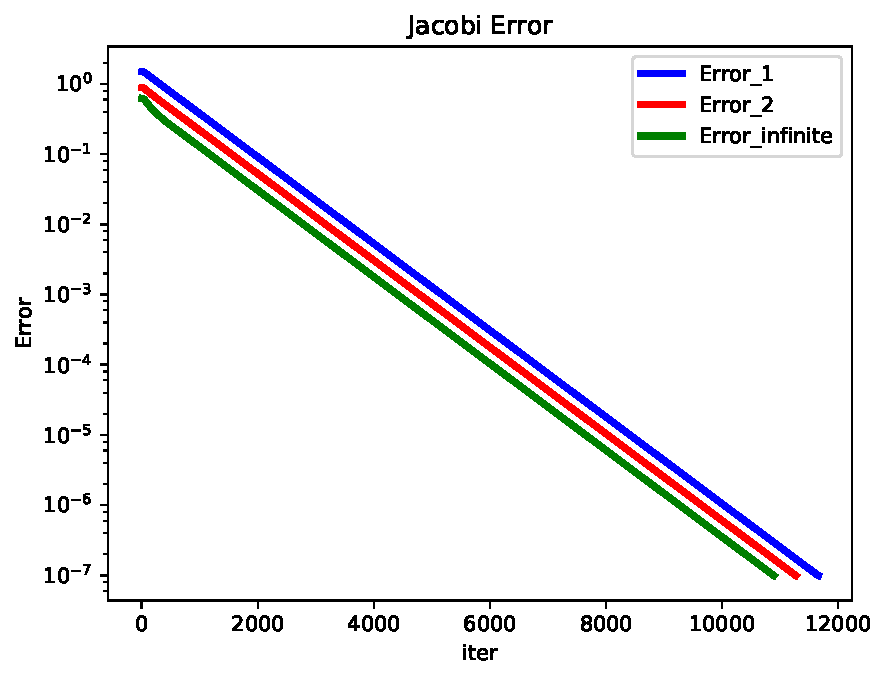
\includegraphics[width=0.7\textwidth]{src/jacobi_error.pdf}
    \caption{Error drop of Jacobi Method}
    \label{fig:jacobi_error}
\end{figure}
\begin{figure}[H]
    \centering
    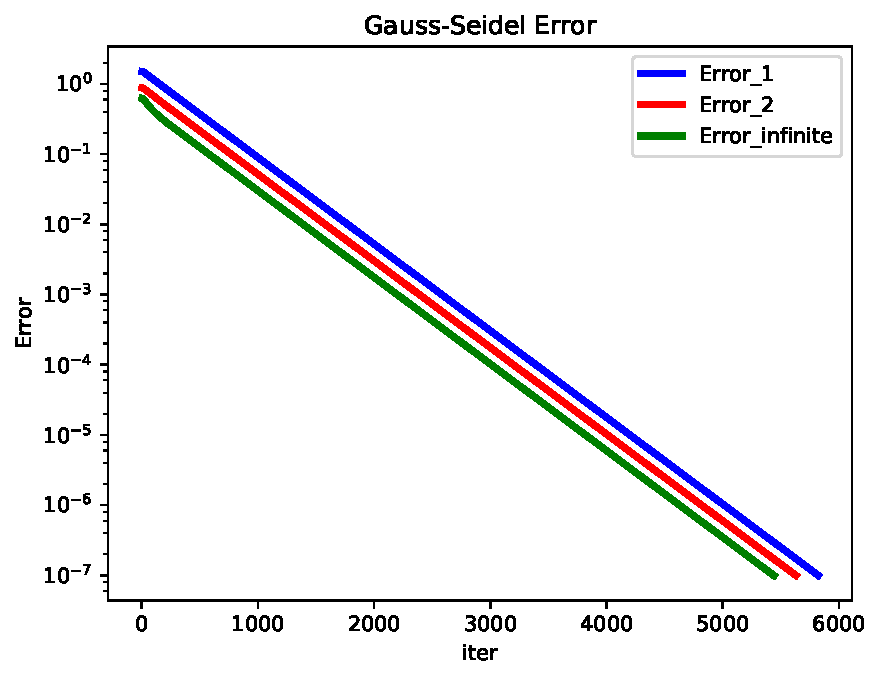
\includegraphics[width=0.7\textwidth]{src/gauss_error.pdf}
    \caption{Error drop of Gauss-Seidel Method}
    \label{fig:gauss_error}
\end{figure}
\begin{figure}[H]
    \centering
    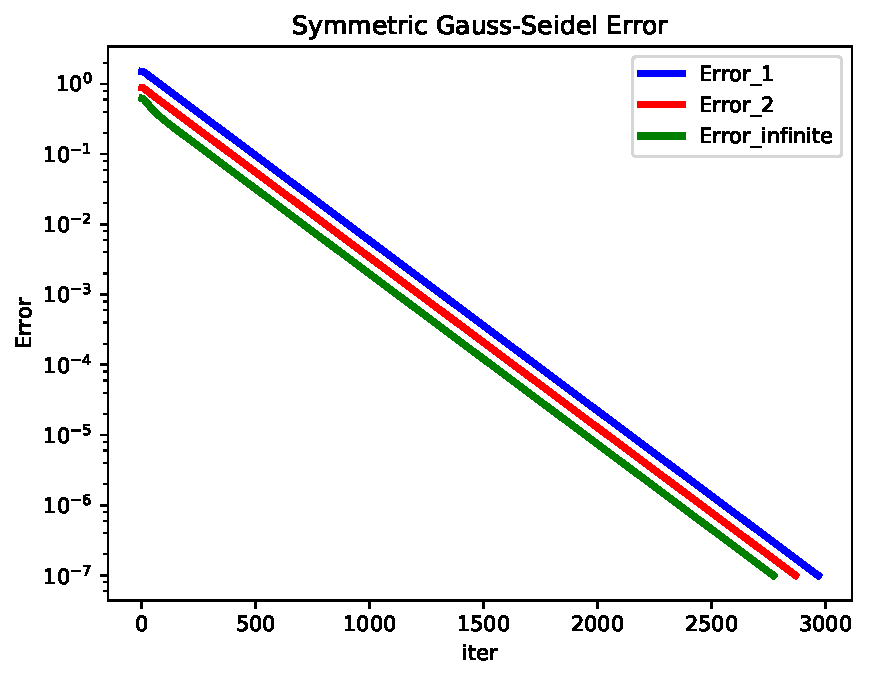
\includegraphics[width=0.7\textwidth]{src/sgs_error.pdf}
    \caption{Error drop of Symmetric Gauss-Seidel Method}
    \label{fig:sgs_error}
\end{figure}
From Figure \ref{fig:jacobi_error}, \ref{fig:gauss_error}, \ref{fig:sgs_error}, we can find that \textbf{Error\_infinite} 
has the fastest convergence rate.

\subsection{Complexity}
From Section \ref{sec:complexity}, we know the complexity of each iteration should be $O(n^2)$. As a result, when we plot 
time vs N, the slope should be same as $n^2$. To verify this, I run several experiment with different N. Table \ref{tab:N} show 
detail result:
\begin{table}[H]
  \centering
    \begin{tabular}{|c|c|c|c|c|c|c|}
    \hline
        & N   & 9   & 25  & 121 & 441 & 1681 \bigstrut\\
    \hline
    \multirow{3}[6]{*}{Jacobi} & iteration & 62  & 310 & 2404 & 10892 & 47614 \bigstrut\\
\cline{2-7}        & runtime(s) & 0.000158 & 0.00118 & 0.146127 & 8.12884 & 532.855 \bigstrut\\
\cline{2-7}        & iter\_avg(s) & 2.54839E-06 & 3.80645E-06 & 6.07849E-05 & 0.000746313 & 0.01119114 \bigstrut\\
    \hline
    \multicolumn{1}{|r}{} & \multicolumn{1}{r}{} & \multicolumn{1}{r}{} & \multicolumn{1}{r}{} & \multicolumn{1}{r}{} & \multicolumn{1}{r}{} &  \bigstrut\\
    \hline
    \multirow{3}[6]{*}{Gauss-Seidel} & iteration & 32  & 155 & 1202 & 5441 & 23779 \bigstrut\\
\cline{2-7}        & runtime(s) & 0.000133 & 0.000586 & 0.075157 & 4.06437 & 251.868 \bigstrut\\
\cline{2-7}        & iter\_avg(s) & 4.15625E-06 & 3.78065E-06 & 6.25266E-05 & 0.00074699 & 0.01059203 \bigstrut\\
    \hline
    \multicolumn{1}{|r}{} & \multicolumn{1}{r}{} & \multicolumn{1}{r}{} & \multicolumn{1}{r}{} & \multicolumn{1}{r}{} & \multicolumn{1}{r}{} &  \bigstrut\\
    \hline
    \multirow{3}[6]{*}{Symmetric Gauss-Seidel} & iteration & 23  & 90  & 628 & 2773 & 12007 \bigstrut\\
\cline{2-7}        & runtime(s) & 0.000163 & 0.000691 & 0.079197 & 4.103 & 259.473 \bigstrut\\
\cline{2-7}        & iter\_avg(s) & 7.08696E-06 & 7.67778E-06 & 0.00012611 & 0.001479625 & 0.02161014 \bigstrut\\
    \hline
    \end{tabular}%
  \caption{Result of different N}
  \label{tab:N}%
\end{table}%

From Table \ref{tab:N}, Figure \ref{fig:complexity} show iter\_avg vs N with log-scale:
\begin{figure}[H]
    \centering
    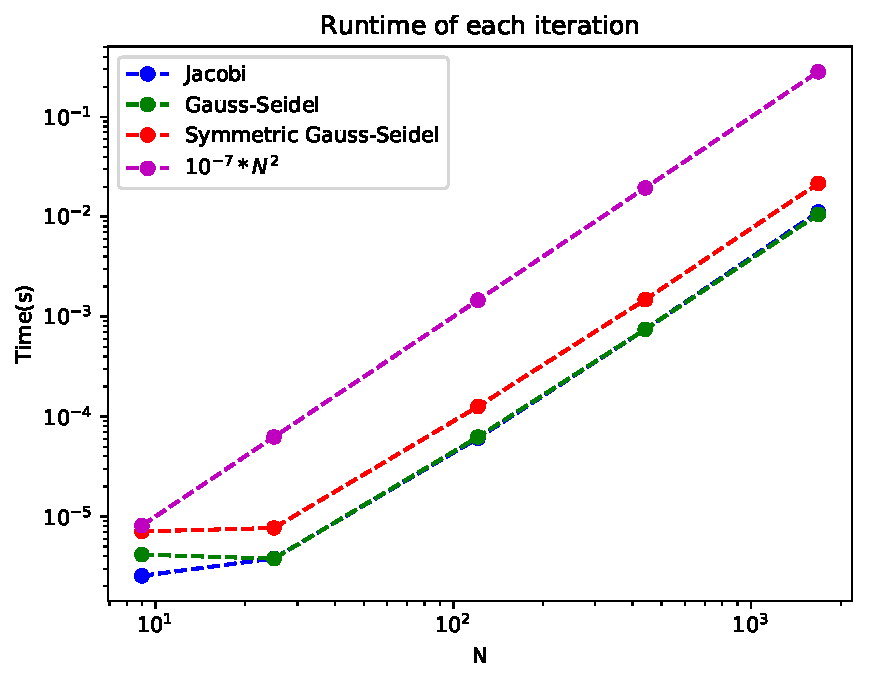
\includegraphics[width=0.8\textwidth]{src/complexity.pdf}
    \caption{Iteration runtime}
    \label{fig:complexity}
\end{figure}
For more clear visualization, I plot $10^{-7} * N^2$ vs N instead of $N^2$ vs N. In Figure \ref{fig:complexity}, we can clearly see
that the slope of three iteration methods are same as $N^2$, which mean their complexity is exactly $O(n^2)$ and satisfy 
my analysis in Section \ref{sec:complexity}.

\subsection{Gauss-Seidel vs Symmetric Gauss-Seidel}
\label{sec:gauss vs sgs}
From Table \ref{tab:N}, we can found that the number of iteration of Gauss-Seidel is almost double as Symmetric Gauss-Seidel 
as shown in Figure \ref{fig:gauss vs sgs iter}:
\begin{figure}[H]
    \centering
    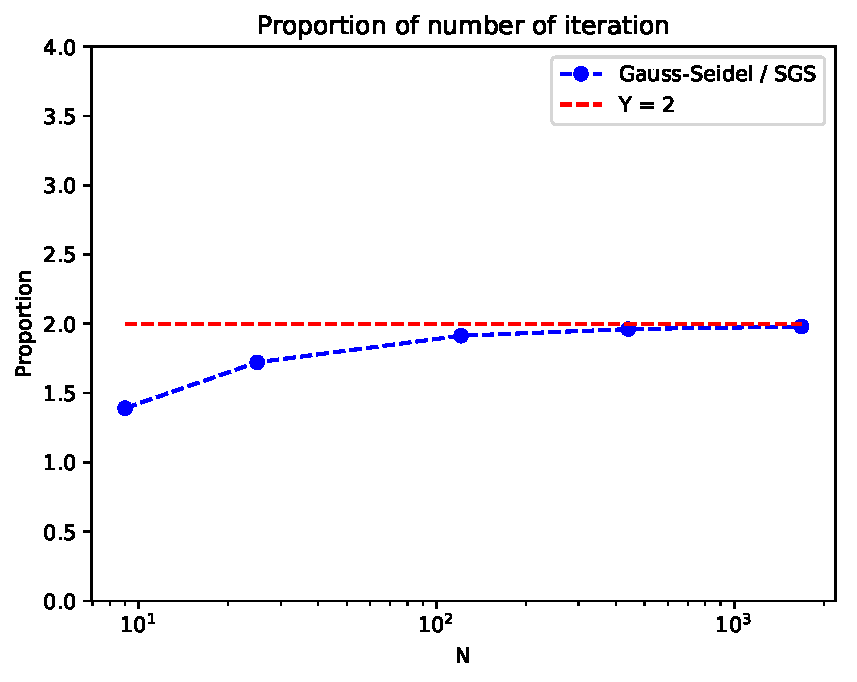
\includegraphics[width=0.7\textwidth]{src/gauss_sgs_iter.pdf}
    \caption{Iteration runtime}
    \label{fig:gauss vs sgs iter}
\end{figure}
Figure \ref{fig:gauss vs sgs iter} exactly shows that Symmetric Gauss-Seidel only use $\frac{1}{2}$ iterations as Gauss-Seidel.
However, when we plot proportion of iter\_avg vs N, we will find that the runtime of each iteration of Symmetric Gauss-Seidel is
double as that of Gauss-Seide, as shown in Figure \ref{fig:gauss vs sgs avg}:
\begin{figure}[H]
    \centering
    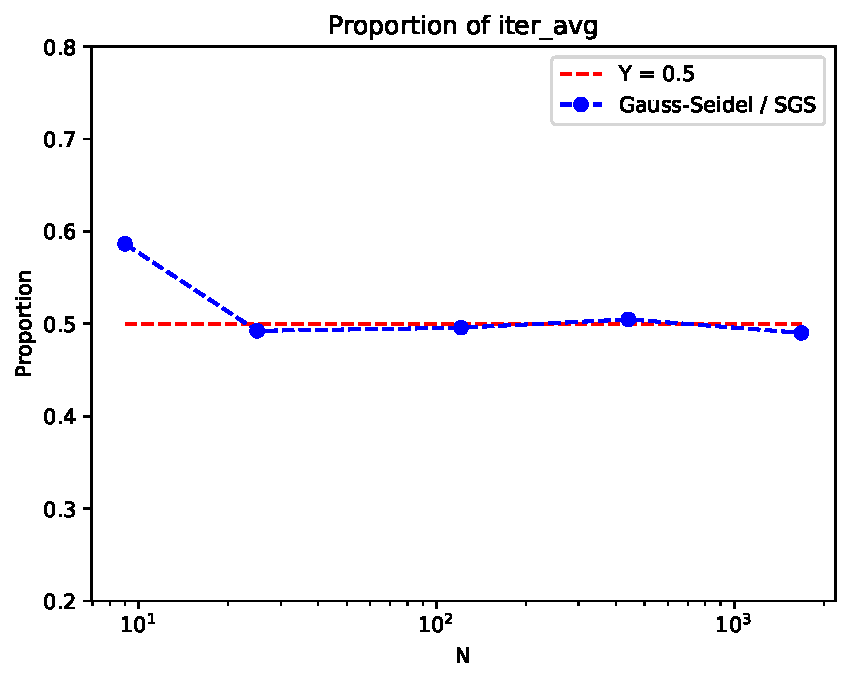
\includegraphics[width=0.7\textwidth]{src/gauss_sgs_avg.pdf}
    \caption{Iteration runtime}
    \label{fig:gauss vs sgs avg}
\end{figure}
As a result, the efficiency of Symmetric Gauss-Seidel is almost same as Gauss-Seidel. When we plot the proportion of total runtime vs N,
we will see it converges to 1, as shown in Figure \ref{fig:gauss vs sgs runtime}:
\begin{figure}[H]
    \centering
    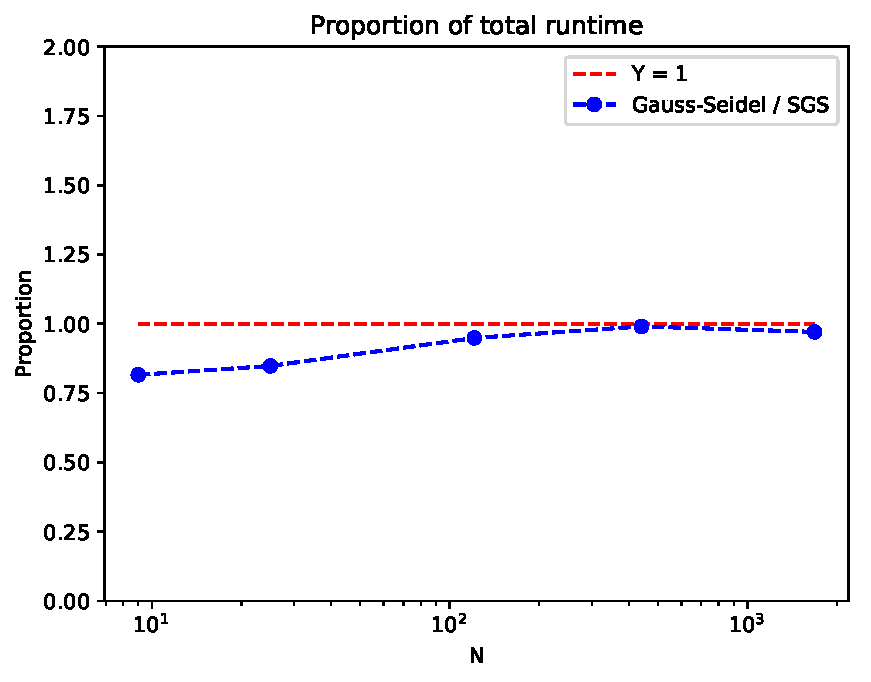
\includegraphics[width=0.7\textwidth]{src/gauss_sgs_runtime.pdf}
    \caption{Iteration runtime}
    \label{fig:gauss vs sgs runtime}
\end{figure}
From Figure \ref{fig:gauss vs sgs runtime}, we can find that Symmetric Gauss-Seidel is actually a little slower than Gauss-Seidel.
As a result, Gauss-Seidel Method is better than Symmetric Gauss-Seidel.

\subsection{Comparison}
\label{sec:comparison}
From Table \ref{tab:N}, iter\_avg of Jacobi and Gauss-Seidel are almost same, but iteration number of jacobi is larger than
Gauss-Seidel. And from Section \ref{sec:gauss vs sgs}, we know Gauss-Seidel is better than Symmetric Gauss-Seidel. As a result, 
Gauss-Seidel is the best algorithm in this homework.


\section{Conclusion}
As we discuss in Section \ref{sec:error} and Section \ref{sec:comparison}, Infinite Error and Gauss-Seidel should be the best 
method in this project.


\end{document}













